\documentclass[runningheads]{llncs}

\usepackage[T1]{fontenc}
\usepackage{graphicx}
\usepackage{booktabs}
\usepackage{tabularx}
\usepackage{multirow}
\usepackage{amsmath}
\usepackage{amssymb}
\usepackage{xcolor}
\usepackage{url}
\usepackage{hyperref}
\usepackage{enumitem}

\hypersetup{
  colorlinks=true,
  linkcolor=blue,
  citecolor=blue,
  urlcolor=blue
}

\title{Unified Coarse-to-Fine Landmark Localization for Multi-Domain Ultrasound Biometry}

\titlerunning{Unified Coarse-to-Fine Ultrasound Biometry}

\author{
Hamza Rasaee\inst{1}
\and
Hassan Rivaz\inst{1}
}

\authorrunning{H. Rasaee and H. Rivaz}

\institute{
Department of Electrical and Computer Engineering, Concordia University, Montreal, Canada\\
\email{\{hamza.rasaee,hassan.rivaz\}@concordia.ca}
}

\begin{document}
\maketitle

\begin{abstract}
\noindent Accurate ultrasound biometry depends on precise anatomical landmark localization across heterogeneous imaging domains. This problem is challenging because ultrasound appearance, field of view, and landmark geometry vary substantially across anatomies, acquisition protocols, and devices. We present a unified multi-task landmark localization framework for multi-domain ultrasound biometry that combines a pretrained DINOv3 encoder with coarse-to-fine decoding, task-conditioned feature aggregation, and heatmap-based prediction within a single model. The framework is designed to preserve global anatomical context while maintaining the local precision required for clinically meaningful measurements. We study the effects of backbone scaling, feature sharing, decoder specialization, and validation design under a common training and evaluation pipeline. The strongest local model, based on a DINOv3 ViT-L backbone with task-specific feature pyramids, achieves an average mean radial error of 11.00 pixels, while a grouped-validation variant of the DINOv3 ViT-B model achieves 11.35 pixels under a stricter selection regime. Our experiments show that stronger pretrained representations can substantially improve local landmark localization, but robust cross-domain generalization remains the key bottleneck. These results support unified coarse-to-fine modeling as a practical direction for robust ultrasound biometry across anatomies and devices.

\keywords{Ultrasound Biometry \and Multi-Task Learning \and DINOv3 \and Landmark Localization \and Vision Transformers}
\end{abstract}

\section{Introduction}
This paper addresses the problem of building a single ultrasound landmark localization model that remains accurate across heterogeneous anatomies, acquisition protocols, and devices while still producing clinically meaningful biometric measurements. In the Foundation Model for Ultrasound Biometry benchmark, one submission must process fetal, intrapartum, and adult cardiac ultrasound with substantially different appearance and geometry. Some subsets require only two endpoints, whereas others require dense multi-landmark configurations over a wide field of view. This setting makes anatomy-specific pipelines inconvenient and motivates a unified model that can share representation learning while still adapting to task-specific landmark structure.

Our goal in this work is not only to reduce landmark error on a local validation split, but to develop a single-model pipeline that better matches the official challenge objective. The benchmark ranking combines normalized mean radial error (MRE) and normalized parameter prediction error with equal weight, so good performance requires both precise landmark localization and geometrically consistent predictions for downstream measurements. During development, this exposed a central difficulty: models that looked strong under one local selection criterion did not always remain strong under stricter validation settings. The paper therefore focuses on the model and training decisions that were most relevant to this gap.

We build the study around a unified DINOv3-based multi-task architecture with challenge-compliant preprocessing, task-conditioned heatmap prediction, soft-argmax coordinate decoding, and measurement-aware analysis. Within this framework, we investigate backbone scaling, shared versus task-specific feature pyramids, decoder specialization, canonical ordering for paired landmarks, and validation strategies aimed at improving hidden-domain robustness. The resulting system is a single challenge-ready model rather than an ensemble or a collection of anatomy-specific networks. More concretely, this paper makes four contributions. First, we formulate all nine Foundation Model for Ultrasound Biometry subsets within one challenge-compliant landmark pipeline with shared preprocessing, shared representation learning, and task-conditioned decoding. Second, we develop a unified coarse-to-fine DINOv3-based architecture with task-specific feature aggregation and heatmap decoding for heterogeneous ultrasound landmark geometry. Third, we provide an empirical study of the design choices that actually shaped the final system, including backbone scaling, FPN sharing, decoder specialization, and paired-landmark canonicalization. Fourth, we analyze the mismatch between easier and stricter local validation settings, showing that robustness remains the main barrier to stronger generalization.

\section{Related Work}
Automated ultrasound biometry has often been studied through anatomy-specific pipelines for fetal head, abdomen, long-bone, and cardiac measurements~\cite{baumgartner2017sononet,isuog2019biometry}. For the setting studied in this paper, however, the key problem is not only anatomy recognition but precise landmark localization across multiple domains. Landmark-based formulations are especially attractive because the same predicted points can be evaluated geometrically and converted into downstream biometric measurements~\cite{payer2016regressing,payer2019integrating}. This makes landmark localization a natural common representation for a benchmark that mixes line-like, diameter-like, and dense multi-point tasks.

Our method is most directly related to heatmap-based keypoint localization. Stacked hourglass networks, HRNet, and CenterNet-style formulations showed that dense spatial supervision remains highly effective for accurate point prediction~\cite{newell2016hourglass,sun2019hrnet,zhou2019objects}. Structured landmark models further indicate that explicit spatial reasoning helps when appearance cues are weak or ambiguous~\cite{payer2019integrating}. These observations are particularly relevant in ultrasound, where speckle, acoustic shadowing, and low-contrast boundaries can make direct coordinate regression unstable.

The shared encoder in our model is motivated by recent self-supervised vision transformers. ViT, Swin Transformer, MAE, BYOL, DINO, DINOv2, and DINOv3 have shown that large-scale pretrained representations transfer effectively across tasks and domains~\cite{dosovitskiy2021vit,liu2021swin,he2022mae,grill2020byol,caron2021dino,oquab2024dinov2}. Rather than training separate models for each subset, we use this line of work to justify a shared representation backbone for all nine tasks and then study how much specialization is still needed in the neck and decoder.

Our training design is also connected to multi-task learning. Hard parameter sharing, soft parameter sharing, cross-stitch style feature exchange, and uncertainty-based weighting have all been proposed to balance related but non-identical objectives~\cite{caruana1997,ruder2017overview,misra2016crossstitch,kendall2018multitask}. The Foundation Model for Ultrasound Biometry setting is a concrete example of this trade-off: all tasks come from the same imaging modality, but the landmark count, spatial layout, and measurement semantics differ substantially. This motivates our comparison of shared backbones with task-specific feature aggregation and task-conditioned decoding in a single challenge-ready model.

\section{Method}
\subsection{Problem formulation}
Each training image belongs to one of nine tasks:
\texttt{A4C}, \texttt{AOP}, \texttt{FA}, \texttt{FUGC}, \texttt{HC}, \texttt{IVC}, \texttt{PLAX}, \texttt{PSAX}, or \texttt{fetal\_femur}. The number of landmarks ranges from two to twenty-two depending on the anatomy. We cast all tasks into a common heatmap-based landmark regression framework. Task identity determines the number of active landmarks, the output head, and any optional auxiliary losses, while the rest of the training pipeline remains shared.

\subsection{Model overview}
Our unified framework uses a shared pretrained DINOv3 encoder, followed by either a shared or task-specific feature pyramid neck, a task-conditioned heatmap head for each dataset subset, differentiable soft-argmax decoding for coordinate extraction, and optional geometry-aware auxiliary supervision for selected tasks. The main design principle is coarse-to-fine prediction. Deep encoder features provide task-relevant global context, while the neck and heatmap head progressively recover spatial detail for final landmark localization. Figure~\ref{fig:overview} summarizes the unified multi-task setup.

\begin{figure}[t]
  \centering
  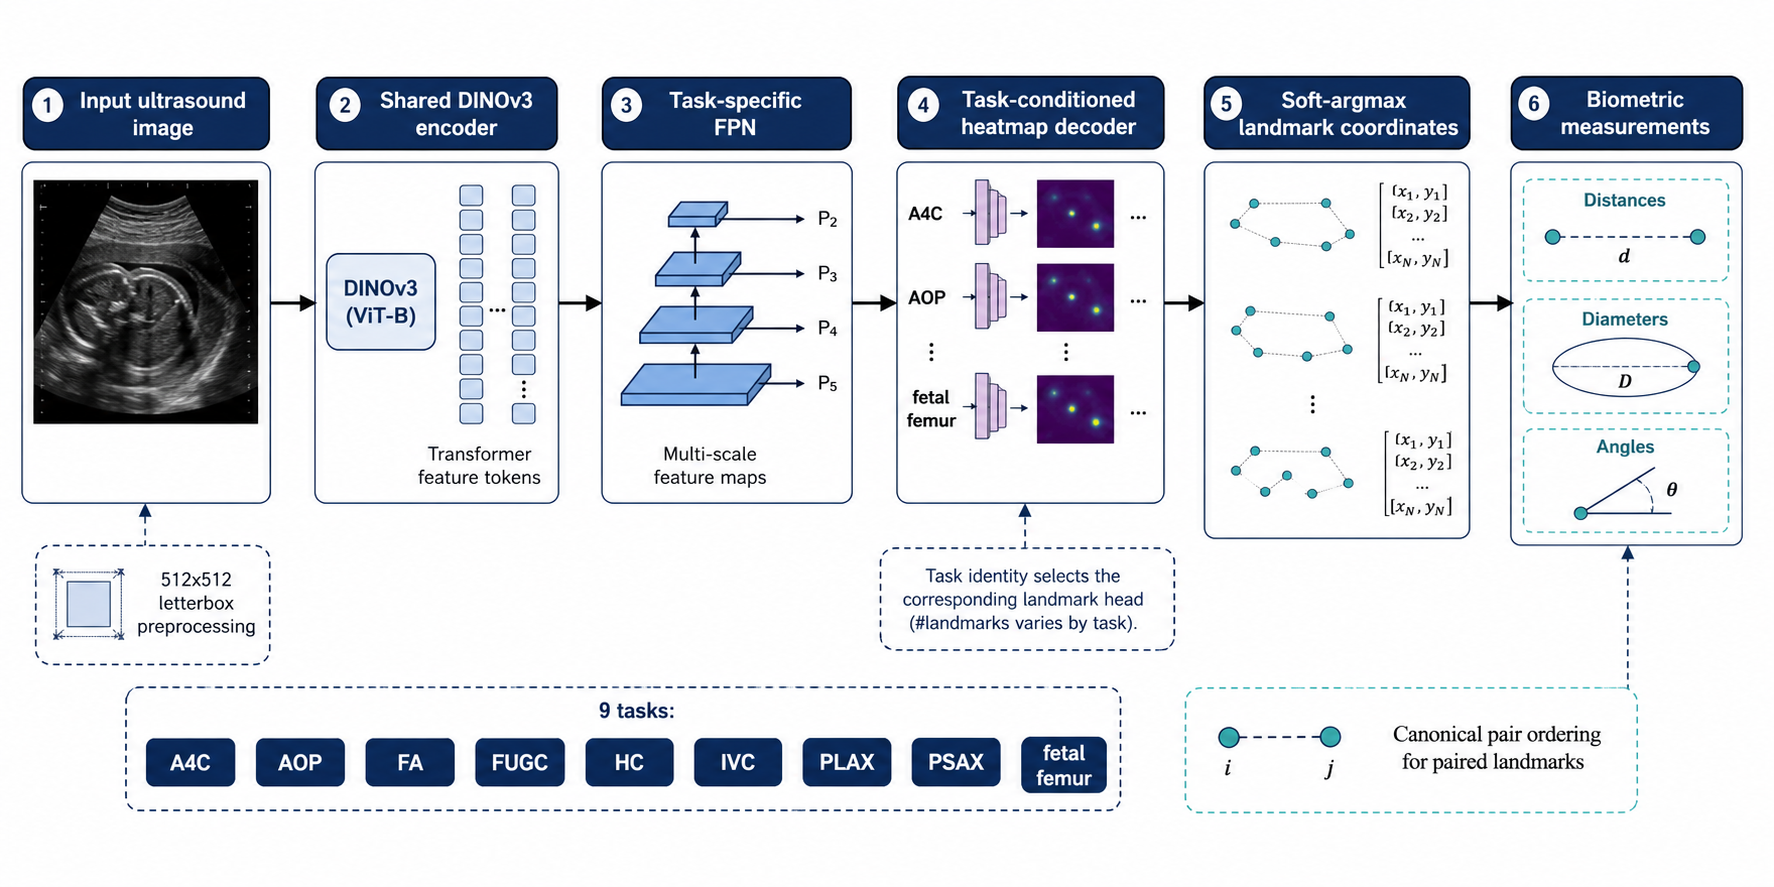
\includegraphics[width=\textwidth]{assets/method_overview_generated_v1.png}
  \caption{Method overview of the proposed multi-domain ultrasound biometry model. A shared DINOv3 encoder is followed by a task-specific FPN, task-conditioned heatmap decoding, soft-argmax coordinate extraction, and measurement derivation, with canonical ordering enforced for paired-landmark tasks.}
  \label{fig:overview}
\end{figure}

\subsection{Shared backbone and feature neck}
Our main model family uses a pretrained DINOv3 visual transformer as the shared encoder. We initially used a ViT-B backbone and later added support for \texttt{vit\_large\_patch16\_dinov3}. To keep the larger model practical, training uses mixed precision and gradient accumulation.

On top of the encoder, we use either a shared FPN or a task-specific FPN. The task-specific variant consistently performed better in our experiments. We attribute this to the strong geometric mismatch between challenge subsets: dense cardiac landmarking, compact ring-like structures, and short endpoint tasks require different balances between semantic context and local detail.

\subsection{Task-specific decoding}
We investigated several decoder families, including a uniform deep heatmap head shared across all tasks except for output dimensionality, geometry-aware variants for line-like, compact, dense, and femur-like structures, fully dedicated per-task decoders, and soft-sharing adapters that partially separate related task groups. The most reliable behavior across local validation settings came from a comparatively simple configuration with a strong shared backbone, task-specific FPNs, and uniform deep decoders. More aggressive specialization often improved selected tasks on local validation but reduced overall robustness. This suggests that anatomical inductive bias is useful only when it does not overfit subset-specific shortcuts in the released training distribution.

\subsection{Training objectives}
The final model is trained with a base landmark loss that combines dense heatmap supervision and direct coordinate supervision:
\begin{equation}
\mathcal{L}_{\text{base}} =
\mathcal{L}_{\text{heatmap}} + 0.2 \mathcal{L}_{\text{coord}}.
\end{equation}

Here, $\mathcal{L}_{\text{heatmap}}$ supervises the predicted landmark heatmaps at the output resolution, while $\mathcal{L}_{\text{coord}}$ penalizes the difference between soft-argmax landmark coordinates and the reference coordinates in image space. This combination gives the model both dense spatial guidance and direct point-level refinement. In our final configuration, the heatmap term provides the main localization signal and the coordinate term sharpens the final landmark positions.

For geometry-sensitive subsets, the training framework also supports task-aware auxiliary supervision based on clinically meaningful structures such as short segments and long-bone shafts. This allows the optimization to remain aligned with the measurement geometry of the underlying anatomy while preserving a single unified landmark-learning objective across all tasks.

\subsection{Data pipeline}
The released datasets were standardized into a common CSV schema to support unified loading, preprocessing, and submission generation. Images are resized with aspect-ratio-preserving letterboxing so that coordinate transforms remain consistent across training, evaluation, and JSON export.

A practically important issue was task-specific ordering ambiguity for paired landmarks. To avoid supervision noise in two-point and paired-diameter tasks, we introduced canonical pair ordering for subsets such as \texttt{FUGC}, \texttt{IVC}, \texttt{AOP}, \texttt{FA}, \texttt{HC}, \texttt{PSAX}, and \texttt{fetal\_femur}. This stabilizes both optimization and derived measurement consistency.

\section{Experiments and Results}
\subsection{Dataset and evaluation protocol}
All experiments use the public Foundation Model for Ultrasound Biometry release and its nine task subsets~\cite{fubiometrychallenge,fubiometrybaseline}. Local development is performed on a train/validation split derived from the released annotations. Because hidden-test labels are unavailable, we report local MRE as the primary development metric and also monitor derived measurement error where possible. The official evaluation combines landmark MRE and clinically derived parameter error with normalized aggregation. To better reflect this setting, we additionally introduced grouped validation splits and weighted checkpoint selection that emphasize historically difficult local subsets.

\subsection{Implementation details}
Images are resized to 512\,$\times$\,512 with letterboxing, and heatmaps are predicted at 64\,$\times$\,64 resolution. Models are optimized with AdamW and cosine learning-rate decay. We use mixed precision, exponential moving average checkpoints, and early stopping. Training and evaluation were performed on NVIDIA RTX 4090 GPUs with 24\,GB memory. For larger backbones, gradient accumulation is used to maintain an effective batch size without exceeding GPU memory.

\subsection{Main results}
We report local validation results on the released data split. Table~\ref{tab:main-results} compares representative architecture variants from the current study and the earlier project line under their respective local evaluation settings. In addition to the strongest row-split local model, we include the grouped-validation ViT-B variant because it was developed specifically to better stress hidden-domain robustness during model selection.

\begin{table}[t]
  \centering
  \caption{Local validation comparison of representative model variants.}
  \label{tab:main-results}
  \small
  \begin{tabularx}{\textwidth}{p{3.2cm} p{2.0cm} X c}
    \toprule
    Method variant & Backbone & Architectural characteristics & Average MRE$\downarrow$ (px) \\
    \midrule
    Unified model & DINOv3 ViT-B & task-specific FPN with uniform deep heatmap decoders & 11.77 \\
    Grouped-validation model & DINOv3 ViT-B & task-specific FPN under grouped-validation selection & 11.35 \\
    Unified model & DINOv3 ViT-L & task-specific FPN with uniform deep heatmap decoders & \textbf{11.00} \\
    \midrule
    Earlier unified DINO baseline & DINOv3-B & coarse-to-fine decoder & 23.05 \\
    Earlier enhanced DINO model & DINOv3-B & dual-branch heads with local refinement & 22.53 \\
    Earlier ConvNeXt--ResNet hybrid & ConvNeXtV2 + ResNet101d & fused dual-encoder decoder & 22.85 \\
    Earlier iterative DINO model & DINOv3-B & iterative refinement decoder & 25.26 \\
    \bottomrule
  \end{tabularx}
\end{table}

The best local result in the current study was obtained with the DINOv3 ViT-L backbone and task-specific FPN. For this model, per-task MRE values were 14.04 for \texttt{A4C}, 6.70 for \texttt{AOP}, 8.72 for \texttt{FA}, 4.02 for \texttt{FUGC}, 13.37 for \texttt{HC}, 16.71 for \texttt{IVC}, 11.21 for \texttt{PLAX}, 13.91 for \texttt{PSAX}, and 10.36 for \texttt{fetal\_femur}. Under the stricter grouped-validation protocol, the DINOv3 ViT-B grouped-selection model reached 11.35 average MRE with per-task values of 18.05 for \texttt{A4C}, 7.32 for \texttt{AOP}, 9.89 for \texttt{FA}, 4.34 for \texttt{FUGC}, 11.61 for \texttt{HC}, 16.34 for \texttt{IVC}, 11.62 for \texttt{PLAX}, 13.92 for \texttt{PSAX}, and 9.04 for \texttt{fetal\_femur}. Relative to the earlier project line, the current architecture family provides a substantial reduction in average local MRE, indicating the benefit of stronger pretrained representations together with cleaner task-specific feature aggregation. At the same time, the grouped-validation result is important because it shows that a slightly weaker local score can emerge from a more demanding selection regime intended to better reflect hidden-domain deployment.

\begin{figure}[t]
  \centering
  \begin{minipage}[t]{0.48\textwidth}
    \centering
    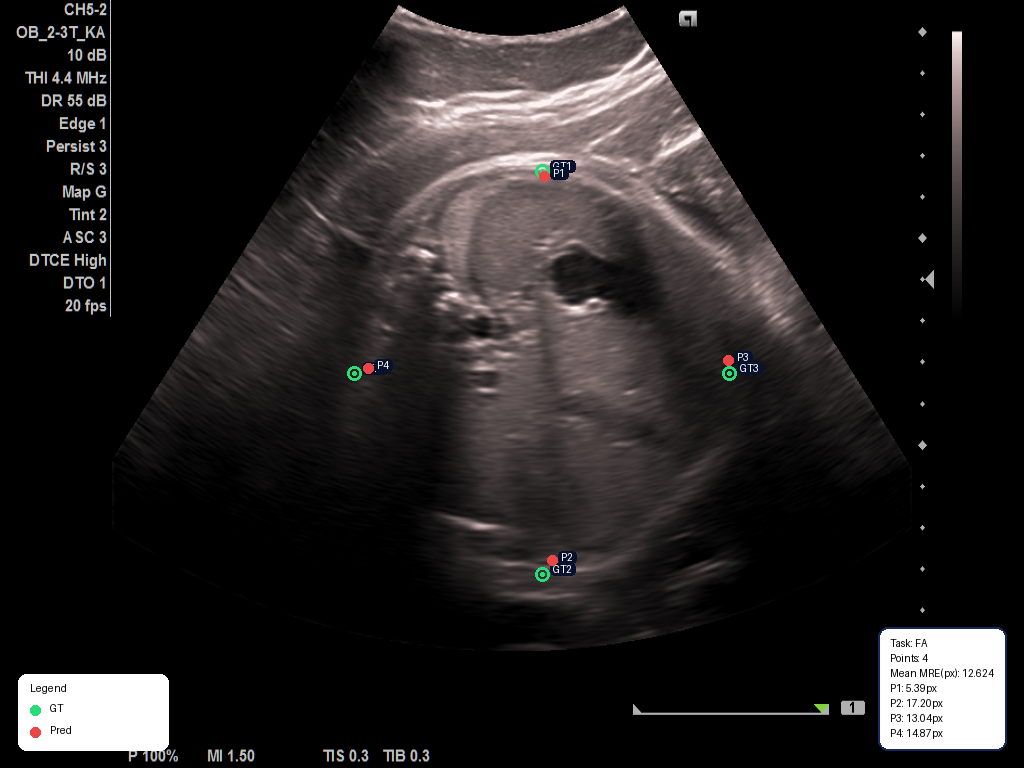
\includegraphics[width=\linewidth,height=4.0cm]{assets/qual_fa.png}
  \end{minipage}\hfill
  \begin{minipage}[t]{0.48\textwidth}
    \centering
    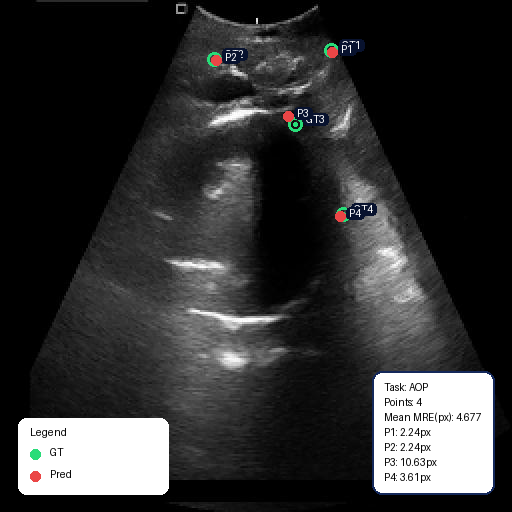
\includegraphics[width=\linewidth,height=4.0cm]{assets/qual_aop.png}
  \end{minipage}
  \caption{Qualitative examples. Ground-truth landmarks are shown in green and predictions in red. Left: fetal-abdomen landmarks with close spatial agreement. Right: accurate endpoint localization on an AOP sample.}
  \label{fig:qualitative_results}
\end{figure}

\subsection{Ablation findings}
The ablation study showed several consistent patterns. Task-specific FPNs were better than a shared FPN across multiple runs and backbone sizes. Larger backbones improved local validation, with the DINOv3 ViT-L model producing our best row-split local MRE of 11.00. However, the grouped-validation ViT-B configuration remained competitive at 11.35 while being selected under a substantially stricter regime. Decoder quality also mattered more than naive refinement depth: in the earlier project line, an enhanced dual-branch DINOv3-B model reached 22.53 average MRE, outperforming an iterative refinement variant at 25.26 average MRE. At the same time, more specialization was not always better, because dedicated heads and task-specific auxiliary losses sometimes improved one or two subsets while hurting overall robustness. The dominant lesson of the study was that local validation must be designed carefully to avoid optimistic conclusions.

\section{Discussion}
The main remaining gap is robust cross-domain generalization under scanner, device, and acquisition shifts. The DINOv3 ViT-L model reduced local landmark error, but the sensitivity of results to validation design indicates that a simple row-level split can still underestimate generalization difficulty. The grouped-validation ViT-B result at 11.35 MRE is therefore informative even though it does not beat the best row-split local score, because it was obtained under a stricter selection regime intended to better penalize unstable subset behavior. Unified multi-task modeling remains viable, but model selection must use a stronger validation regime. To address this, we extended the training pipeline with grouped validation splits derived from study- or patient-style filename patterns, stronger ultrasound-style augmentation, and weighted checkpoint selection that emphasized difficult local subsets such as \texttt{IVC}, \texttt{A4C}, and \texttt{HC}. These changes aim to reduce overfitting to the released training distribution and align local model selection more closely with the evaluation objective.

\section{Limitations and Future Work}
Local validation remains an approximation of full cross-domain generalization, and challenge-normalized measurement quality is only partially reflected by our current local selection metric. In addition, all experiments are constrained to a single submitted model. Future work should emphasize stronger domain generalization, measurement-aware local validation, and more principled feature-sharing or task-balancing mechanisms~\cite{caruana1997,kendall2018multitask,misra2016crossstitch}.

\section{Conclusion}
We presented a unified coarse-to-fine landmark localization framework for multi-domain ultrasound biometry based on shared DINOv3 features and task-conditioned heatmap decoding. Our strongest local model achieved 11.00 average MRE with a DINOv3 ViT-L backbone, and a grouped-validation DINOv3 ViT-B variant achieved 11.35 average MRE under a stricter selection protocol. The main conclusion is that stronger pretrained representations help, but robust performance depends just as strongly on domain-aware validation and challenge-aligned model selection.

\section*{Acknowledgments}
This study used the public Foundation Model for Ultrasound Biometry data release and baseline repository provided by the challenge organizers. Training and evaluation were performed on NVIDIA RTX 4090 GPUs.

\bibliographystyle{splncs04}
\bibliography{references}

\end{document}
